%Evaluación N°1. Generado desde report/informe.tex.tpl por scripts/pipeline.sh
% (las cifras provienen de report/valores.env). Compilar con: xelatex informe.tex (dos veces) o latexmk -xelatex.
\documentclass[11pt,a4paper]{article}
\usepackage{fontspec}
\usepackage[spanish,es-noshorthands,es-tabla]{babel}
\usepackage[a4paper,margin=2.4cm]{geometry}
\usepackage{booktabs,graphicx,float,adjustbox,caption,xcolor,enumitem,listings,fancyhdr,setspace}
\usepackage[hidelinks]{hyperref}
\usepackage{amsmath}
\usepackage{underscore}   % permite _ dentro de \texttt sin escapar
\captionsetup{font=small,labelfont=bf}
\setlist{itemsep=2pt,topsep=4pt}
\setstretch{1.08}
\emergencystretch=3em      % evita desbordes por palabras largas en \texttt
\lstset{basicstyle=\ttfamily\footnotesize,breaklines=true,columns=fullflexible,frame=single,
  backgroundcolor=\color{black!4},rulecolor=\color{black!20},xleftmargin=2pt,xrightmargin=2pt,
  showstringspaces=false,upquote=true}
\newcommand{\cod}[1]{\texttt{#1}}
\newenvironment{tablaentex}[2]{% caption, label; el contenido (tabular) lo inserta el pipeline
  \begin{table}[H]\centering\small\caption{#1}\label{#2}\begin{adjustbox}{max width=\textwidth}}%
  {\end{adjustbox}\end{table}}
\pagestyle{fancy}\fancyhf{}
\fancyhead[L]{\small Evaluación N°1}
\fancyhead[R]{\small Dataset: Diabetes}
\fancyfoot[C]{\thepage}
\renewcommand{\headrulewidth}{0.3pt}

\begin{document}

% ------------------------------------------------------------------ PORTADA
\begin{titlepage}
\centering
{\large UNIVERSIDAD DEL BÍO-BÍO}\\[2pt]
{\normalsize Facultad de Ciencias}\\[2pt]
{\normalsize Departamento de Estadística}\\[1.6cm]
\rule{\textwidth}{0.6pt}\\[0.5cm]
{\Large\bfseries Ciencia de Datos en la Terminal Linux}\\[0.4cm]
{\large Evaluación N°1}\\[0.5cm]
\rule{\textwidth}{0.6pt}\\[1.6cm]
{\LARGE\bfseries ¿Quién vuelve al hospital?}\\[0.5cm]
{\Large Reingresos de pacientes diabéticos en 130 hospitales de EE.\,UU.}\\[1.2cm]
{\large Dataset asignado: \textbf{Diabetes}}\\[2.2cm]
\begin{tabular}{rl}
\textbf{Autora:}   & Trinidad Saez \\
\textbf{Profesor:} & Luis Gómez \\
\textbf{Entrega:}  & 22 de octubre de 2026 \\
\end{tabular}\\[2cm]
{\normalsize Octubre de 2026}
\vfill
{\small Repositorio con el código, el pipeline reproducible y este informe:\\ \texttt{scripts/pipeline.sh} $\cdot$ \texttt{report/reporte.md} $\cdot$ \texttt{report/informe.pdf}}
\end{titlepage}

\tableofcontents
\vspace{1.5em}
\listoffigures
\clearpage
\listoftables
\clearpage

% ------------------------------------------------------------------ 1
\section{Introducción y objetivo}
El comité de calidad de una red hospitalaria quiere reducir los reingresos tempranos de pacientes con diabetes.
Cuenta con un programa de seguimiento telefónico post-alta, pero solo puede contactar al \textbf{20\,\%} de los pacientes.
Con registros de diez años (1999--2008) de atención en 130 hospitales de EE.\,UU., el comité plantea la pregunta:
\begin{quote}\itshape ¿Qué características de un paciente se asocian con un reingreso en menos de 30 días y qué tan bien permite un modelo sencillo priorizar al 20\,\% de pacientes con mayor riesgo?\end{quote}
El trabajo se realizó exclusivamente con herramientas de línea de comandos (\cod{awk}, \cod{sed}, \cod{tr}, \cod{sort}, \cod{csvkit}, \cod{vw}, \cod{python3} con \cod{matplotlib}), en un flujo de obtención, limpieza, exploración, modelación e interpretación, empaquetado en un único \emph{pipeline} reproducible (\cod{scripts/pipeline.sh}).

% ------------------------------------------------------------------ 2
\section{Datos y consideraciones éticas}
\textbf{Fuente.} Clore, J., Cios, K., DeShazo, J., \& Strack, B. (2014). \emph{Diabetes 130-US Hospitals for Years 1999-2008} [Conjunto de datos]. UCI Machine Learning Repository. \url{https://doi.org/10.24432/C5230J}.

\textbf{Estudio que describe los datos.} Strack, B., DeShazo, J.\,P., Gennings, C., Olmo, J.\,L., Ventura, S., Cios, K.\,J., \& Clore, J.\,N. (2014). Impact of HbA1c measurement on hospital readmission rates: Analysis of 70,000 clinical database patient records. \emph{BioMed Research International}, 2014, 781670. \url{https://doi.org/10.1155/2014/781670}.

El archivo \cod{diabetic_data.csv} contiene 101\,766 hospitalizaciones de 71\,518 pacientes (una fila por hospitalización) y 50 columnas: identificadores (\cod{encounter\_id}, \cod{patient\_nbr}), datos demográficos (\cod{race}, \cod{gender}, \cod{age} en intervalos de 10 años), características de la estadía (\cod{time\_in\_hospital}, \cod{num\_lab\_procedures}, \cod{num\_medications}, \dots), visitas del año anterior (\cod{number\_outpatient}, \cod{number\_emergency}, \cod{number\_inpatient}), diagnósticos (\cod{diag\_1}--\cod{diag\_3}, códigos ICD-9), exámenes (\cod{A1Cresult}, \cod{max\_glu\_serum}), 23 columnas de medicamentos, \cod{change}, \cod{diabetesMed} y la respuesta \cod{readmitted} (\cod{<30}, \cod{>30}, \cod{NO}). El archivo \cod{IDS\_mapping.csv} es el diccionario de los códigos \cod{admission\_type\_id}, \cod{discharge\_disposition\_id} y \cod{admission\_source\_id}.

\textbf{Datos sensibles.} Los datos incluyen edad, sexo y raza. Se adoptaron tres decisiones: (i) el repositorio \emph{no} contiene los datos (el \emph{pipeline} los descarga desde UCI); (ii) la \textbf{raza no se usa como predictor}; y (iii) se \textbf{audita} el desempeño del modelo por grupo racial (sección~\ref{sec:equidad}).

% ------------------------------------------------------------------ 3
\section{Metodología}\label{sec:metodo}
\subsection{Entorno y reproducibilidad}
El análisis se ejecuta desde la raíz del repositorio con \cod{bash scripts/pipeline.sh}; todas las rutas son relativas (\cod{./data}, \cod{./scripts}, \cod{./report}). El script usa \cod{set -eu} y verificaciones automáticas (por ejemplo, que \cod{diab\_clean.csv} tenga un paciente por fila y que ningún paciente esté a la vez en entrenamiento y prueba). Las semillas son 42. El apéndice~\ref{app:entorno} lista las versiones del entorno usado. Además, las afirmaciones cualitativas del texto (el orden de los pesos, sus signos, si una tasa «sube» o «baja») se comprueban una a una contra los valores calculados (\cod{data/tablas/verificacion\_texto.csv}, que se genera al ejecutarlo), de modo que el pipeline avisa si alguna deja de cumplirse con otra versión de las herramientas. En esta ejecución se cumplen 31 de 31.

\textbf{Validación entre entornos.} El \emph{pipeline} se ejecutó desde cero, con descarga incluida, en dos entornos con versiones distintas: el contenedor \cod{datasciencetoolbox/dsatcl2e} (\cod{vw} 8.11, \cod{shuf} 8.32, \cod{mawk}, Python 3.9) y Ubuntu 24.04 en WSL (\cod{vw} 8.6.1, \cod{shuf} 9.4, \cod{gawk}, Python 3.12). Todas las tablas, \cod{data/diab\_clean.csv} y \cod{report/valores.env} resultaron idénticos byte a byte. Las probabilidades de \cod{vw} difieren solo en la sexta cifra decimal ($<10^{-5}$), sin cambiar el orden de los pacientes ni ninguna métrica. Solo cambia la línea \emph{Analista} de la ficha, que toma el usuario que ejecuta (\cod{whoami}).

\subsection{Limpieza de datos}
\textbf{Inspección.} Se inspeccionaron los archivos con \cod{head}, \cod{file} y \cod{cat -A}, que muestra los caracteres no imprimibles. Ambos archivos terminan sus líneas en \cod{\^{}M\$} (CRLF), y \cod{IDS\_mapping.csv} reúne tres tablas separadas por líneas con una sola coma. Se normalizaron los terminadores con \cod{tr}; si no se hiciera, el último campo valdría \cod{NO\^{}M} o \cod{<30\^{}M} y cualquier comparación fallaría sin avisar:
\begin{lstlisting}
tr -d '\r' < data/diabetic_data.csv > data/interim/raw_lf.csv
\end{lstlisting}

\textbf{Diccionario.} Se separaron las tres tablas con \cod{awk}: una línea vacía o \cod{,} señala el cambio de tabla, y un encabezado \cod{xxx,description} abre un archivo nuevo. Las descripciones se cortan en la \emph{primera} coma (algunas llevan comas entre comillas) y se les quitan comillas y espacios sobrantes.
\begin{lstlisting}
awk '/^,*$/ {next}
     /^[a-z_]+,description$/ {split($0,h,","); out="data/mapa_" h[1] ".csv"; print > out; next}
     {i=index($0,","); cod=substr($0,1,i-1); d=substr($0,i+1); gsub(/^"|"$/,"",d)
      gsub(/^ +| +$/,"",d); if (d~/,/) d="\"" d "\""; print cod "," d > out}' data/interim/ids_lf.csv
\end{lstlisting}

\textbf{Valores faltantes.} Como el dato faltante no es la celda vacía sino el marcador \cod{?}, se contaron por columna los \cod{?}, las celdas vacías, los \cod{None} y los \cod{Unknown/Invalid} con un \cod{awk} que recorre todas las columnas. Un \cod{None} en \cod{A1Cresult} o \cod{max\_glu\_serum} indica que el examen \emph{no se realizó}; es información clínica y se conserva como categoría. Los códigos del diccionario cuyas descripciones son \cod{NULL}, \cod{Not Available}, \cod{Not Mapped} o \cod{Unknown/Invalid} \emph{son faltantes disfrazados}; se detectan con una expresión regular sobre el propio diccionario (no a mano) y se recodifican como celda vacía junto con los \cod{?}.

\textbf{Exclusión de fallecidos y cuidados paliativos.} Los códigos de alta cuya descripción contiene \cod{Expired} o \cod{Hospice} (11, 13, 14, 19, 20 y 21) se identifican también desde el diccionario y se excluyen. La justificación es distinta para cada grupo. Un paciente \emph{fallecido} no puede reingresar, y dejarlo como «no reingreso» confundiría mortalidad con buena evolución. Un paciente en \emph{hospicio} sí puede reingresar (la tabla~\ref{tab:excl} lo cuantifica), pero pasa a cuidados de fin de vida. Desde ese momento el objetivo clínico ya no es evitar la hospitalización, su reingreso no es un resultado evitable que el programa deba medir y no es candidato a un seguimiento cuyo fin es prevenirlo. Es el mismo criterio de Strack et~al.~(2014).

\textbf{Un registro por paciente.} Se conserva la hospitalización con menor \cod{encounter\_id} de cada paciente:
\begin{lstlisting}
tail -n +2 pasoB.csv | sort -t, -k2,2n -k1,1n | awk -F, '!visto[$2]++' | sort -t, -k1,1n
\end{lstlisting}
La justificación es la independencia: las hospitalizaciones del mismo paciente están correlacionadas y, repartidas entre entrenamiento y prueba, filtrarían información. Además, el programa contacta pacientes y no hospitalizaciones, y los pacientes recurrentes (que reingresan más) dominarían el archivo.

\textbf{Columnas constantes y respuesta.} Una pasada de \cod{awk} cuenta los valores distintos por columna y elimina las que tienen uno solo; en la misma pasada se crea \cod{Reingreso30} $=1$ si \cod{readmitted} es \cod{<30} y $0$ en otro caso. El resultado se guarda en \cod{data/diab\_clean.csv}.

\subsection{Análisis exploratorio}
Las tasas de reingreso por categoría se calculan con \cod{csvcut} (selecciona la variable y \cod{Reingreso30}) y un \cod{awk} que acumula conteos por categoría; los descriptivos (media, desviación estándar, cuartiles, mínimo y máximo) se calculan sobre la columna ordenada. Las figuras se generan con \cod{python3} y \cod{matplotlib} (\cod{scripts/graficos.py}).

\subsection{Modelación predictiva}
\textbf{Modelos.} Regresión logística con Vowpal Wabbit (\cod{vw --loss\_function logistic --passes 10 --l2 1e-6 -b 22}). El \textbf{Modelo A} usa ocho variables numéricas (\cod{time\_in\_hospital}, \cod{num\_lab\_procedures}, \cod{num\_procedures}, \cod{num\_medications}, \cod{number\_outpatient}, \cod{number\_emergency}, \cod{number\_inpatient}, \cod{number\_diagnoses}); el \textbf{Modelo B} agrega \cod{age}, \cod{gender}, \cod{admission\_type\_id}, \cod{admission\_source\_id}, \cod{discharge\_disposition\_id}, \cod{A1Cresult}, \cod{insulin}, \cod{change} y \cod{diabetesMed}, con los códigos tratados como \emph{categorías}. Las numéricas se estandarizan con la media y la desviación estándar del entrenamiento y las categóricas se codifican con \cod{awk} como \cod{variable=valor} (los faltantes como \cod{NA}):
\begin{lstlisting}
-1 |num time_in_hospital:0.219 ... number_diagnoses:0.964 |cat age=_60_70_ gender=Male admission_type_id=NA ...
\end{lstlisting}
\textbf{Partición.} 70\,\% entrenamiento y 30\,\% prueba con semilla 42, sobre \cod{diab\_clean.csv} (una fila por paciente, por lo que la partición es por paciente). El enunciado propone la orden
\begin{lstlisting}
shuf --random-source=<(yes 42)
\end{lstlisting}
Como se muestra en la sección~\ref{sec:resparticion}, esa fuente no mezcla uniformemente, de modo que la partición \emph{principal} usa el mismo comando con una fuente pseudoaleatoria de calidad sembrada con 42 (generador Mersenne Twister de \cod{python3}, \cod{random.Random(42)}), y la del enunciado se conserva como análisis de sensibilidad.

\textbf{Evaluación.} Con las probabilidades $\hat p_i=1/(1+e^{-s_i})$ del conjunto de prueba ($N$ pacientes), se ordena de mayor a menor y se toman los $K=\lfloor N/5\rfloor$ primeros (el 20\,\%). Con $C$ reingresos capturados entre ellos y $T$ reingresos en total:
\[
\text{sensibilidad}=\frac{C}{T},\qquad
\text{precisión}=\frac{C}{K},\qquad
\text{lift}=\frac{C/K}{T/N}.
\]
La selección aleatoria tiene sensibilidad esperada 20\,\% y $\text{lift}=1$. Se agregan: el AUC (Mann--Whitney, con empates), la exactitud con umbral 0.5, una simulación de 1000 selecciones aleatorias del 20\,\%, e intervalos de confianza del 95\,\% por \emph{bootstrap} (1000 remuestras del conjunto de prueba con el corte de puntaje fijo en el del 20\,\% superior).
\begin{lstlisting}
K=$(( NTEST / 5 ))
CAPT=$(tail -n +2 data/test_pred.csv | LC_ALL=C sort -t, -k2,2gr | head -n $K | awk -F, '{s+=$1} END{print s}')
\end{lstlisting}

% 
\section{Resultados}
\subsection{Limpieza}
La tabla~\ref{tab:pasos} resume las filas antes y después de cada paso. Se normalizaron los terminadores de línea y se recodificaron 192\,849 celdas \cod{?} y las celdas con códigos ausentes del diccionario (tabla~\ref{tab:recod}); se excluyeron 2\,423 hospitalizaciones con alta por fallecimiento u hospicio (tabla~\ref{tab:excl}): 1\,652 por fallecimiento, ninguna con reingreso registrado (0), y 771 a hospicio, de las cuales 43 (5.58\,\%) sí reingresaron en menos de 30 días; y se conservó una hospitalización por paciente (29\,353 filas eliminadas). Se eliminaron las columnas constantes \cod{examide}, \cod{citoglipton} y \cod{glimepiride-pioglitazone} (esta última queda constante una vez filtradas las filas). Resultado: 69\,990 pacientes y 48 columnas.

\begin{tablaentex}{Filas, pacientes únicos y columnas después de cada paso de limpieza.}{tab:pasos}
\begin{tabular}{llrrrr}
\toprule
paso & descripcion & filas\_antes & filas\_despues & pacientes\_unicos & columnas \\
\midrule
0 & Archivo original (CRLF -\textgreater{} LF) & 101\,766 & 101\,766 & 71\,518 & 50 \\
A & Recodificar faltantes como vacío & 101\,766 & 101\,766 & 71\,518 & 50 \\
B & Excluir fallecidos y cuidados paliativos & 101\,766 & 99\,343 & 69\,990 & 50 \\
C & Un registro por paciente (primer encounter\_id) & 99\,343 & 69\,990 & 69\,990 & 50 \\
D & Quitar columnas constantes y crear Reingreso30 & 69\,990 & 69\,990 & 69\,990 & 48 \\
\bottomrule
\end{tabular}
\end{tablaentex}
\begin{tablaentex}{Celdas recodificadas como faltantes en el paso A.}{tab:recod}
\begin{tabular}{lr}
\toprule
regla & celdas\_recodificadas \\
\midrule
? -\textgreater{} vacío (todas las columnas) & 192\,849 \\
admission\_type\_id con código ausente & 10\,396 \\
discharge\_disposition\_id con código ausente & 4\,680 \\
admission\_source\_id con código ausente & 7\,067 \\
gender Unknown/Invalid -\textgreater{} vacío & 3 \\
\bottomrule
\end{tabular}
\end{tablaentex}
\begin{tablaentex}{Códigos del diccionario tratados como información ausente o como alta por fallecimiento/paliativos.}{tab:codigos}
\begin{tabular}{lrllr}
\toprule
tabla & codigo & descripcion & clase & filas\_en\_datos \\
\midrule
admission\_type\_id & 5 & Not Available & ausente & 4\,785 \\
admission\_type\_id & 6 & NULL & ausente & 5\,291 \\
admission\_type\_id & 8 & Not Mapped & ausente & 320 \\
discharge\_disposition\_id & 11 & Expired & fallecido\_o\_paliativo & 1\,642 \\
discharge\_disposition\_id & 13 & Hospice / home & fallecido\_o\_paliativo & 399 \\
discharge\_disposition\_id & 14 & Hospice / medical facility & fallecido\_o\_paliativo & 372 \\
discharge\_disposition\_id & 18 & NULL & ausente & 3\,691 \\
discharge\_disposition\_id & 19 & Expired at home. Medicaid only; hospice. & fallecido\_o\_paliativo & 8 \\
discharge\_disposition\_id & 20 & Expired in a medical facility. Medicaid only; hospice. & fallecido\_o\_paliativo & 2 \\
discharge\_disposition\_id & 21 & Expired; place unknown. Medicaid only; hospice. & fallecido\_o\_paliativo & 0 \\
discharge\_disposition\_id & 25 & Not Mapped & ausente & 989 \\
discharge\_disposition\_id & 26 & Unknown/Invalid & ausente & 0 \\
admission\_source\_id & 9 & Not Available & ausente & 125 \\
admission\_source\_id & 15 & Not Available & ausente & 0 \\
admission\_source\_id & 17 & NULL & ausente & 6\,781 \\
admission\_source\_id & 20 & Not Mapped & ausente & 161 \\
admission\_source\_id & 21 & Unknown/Invalid & ausente & 0 \\
\bottomrule
\end{tabular}
\end{tablaentex}
\begin{tablaentex}{Hospitalizaciones excluidas por alta con fallecimiento u hospicio, y cuántas tenían \cod{readmitted} $=$ \cod{<30}.}{tab:excl}
\begin{tabular}{lllrr}
\toprule
codigo & descripcion & tipo & filas\_excluidas & con\_reingreso\_lt30 \\
\midrule
11 & Expired & fallecimiento & 1\,642 & 0 \\
13 & Hospice / home & hospicio & 399 & 19 \\
14 & Hospice / medical facility & hospicio & 372 & 24 \\
19 & Expired at home. Medicaid only; hospice. & fallecimiento & 8 & 0 \\
20 & Expired in a medical facility. Medicaid only; hospice. & fallecimiento & 2 & 0 \\
TOTAL &  &  & 2\,423 & 43 \\
\bottomrule
\end{tabular}
\end{tablaentex}

\textbf{Faltantes y exámenes no realizados.} En el archivo original los porcentajes de \cod{?} fueron: \cod{weight} 96.86\,\%, \cod{medical\_specialty} 49.08\,\%, \cod{payer\_code} 39.56\,\%, \cod{race} 2.23\,\%, \cod{diag\_3} 1.40\,\% y \cod{diag\_2} 0.35\,\%. Los \cod{None} de \cod{A1Cresult} (83.28\,\%) y \cod{max\_glu\_serum} (94.75\,\%) significan examen no realizado y no se imputan. Del diccionario, 10\,396 celdas de \cod{admission\_type\_id}, 4\,680 de \cod{discharge\_disposition\_id} y 7\,067 de \cod{admission\_source\_id} tenían códigos ausentes; \cod{gender} tenía 3 valores \cod{Unknown/Invalid}.

\textbf{Sensibilidad al orden de los pasos.} 1\,545 pacientes tienen como primer encuentro un alta por fallecimiento u hospicio; en 27 de ellos hay encuentros posteriores. Siguiendo el orden del enunciado (excluir y luego dejar uno por paciente) se conserva un encuentro posterior; el caso es marginal (0.04\,\% de los pacientes).

\subsection{Análisis exploratorio}
\paragraph{Respuesta.} En el archivo original el 11.16\,\% de las hospitalizaciones termina en reingreso en menos de 30 días (34.93\,\% a más de 30 días y 53.91\,\% sin reingreso). Tras la limpieza, la tasa de \cod{Reingreso30} es \textbf{8.98\,\%} (6\,285 de 69\,990 pacientes): una clase positiva rara, con desbalance de aproximadamente 1 a 10. Los dos pasos de limpieza mueven la tasa en sentidos opuestos. Excluir fallecidos y hospicio la \emph{sube}, de 11.16\,\% a 11.39\,\% por hospitalización, porque casi todas esas altas tenían \cod{readmitted} $=$ \cod{NO}. Dejar un registro por paciente la \emph{baja} a 8.98\,\%: en el original los pacientes recurrentes, que reingresan más, aportan muchas filas. \cod{Reingreso30} colapsa \cod{>30} y \cod{NO}: mide el reingreso temprano que el programa busca evitar. Predecir siempre «no reingreso» acierta el 90.99\,\% en la prueba, por lo que la exactitud no sirve como métrica (sección~\ref{sec:disc}).

\begin{figure}[H]\centering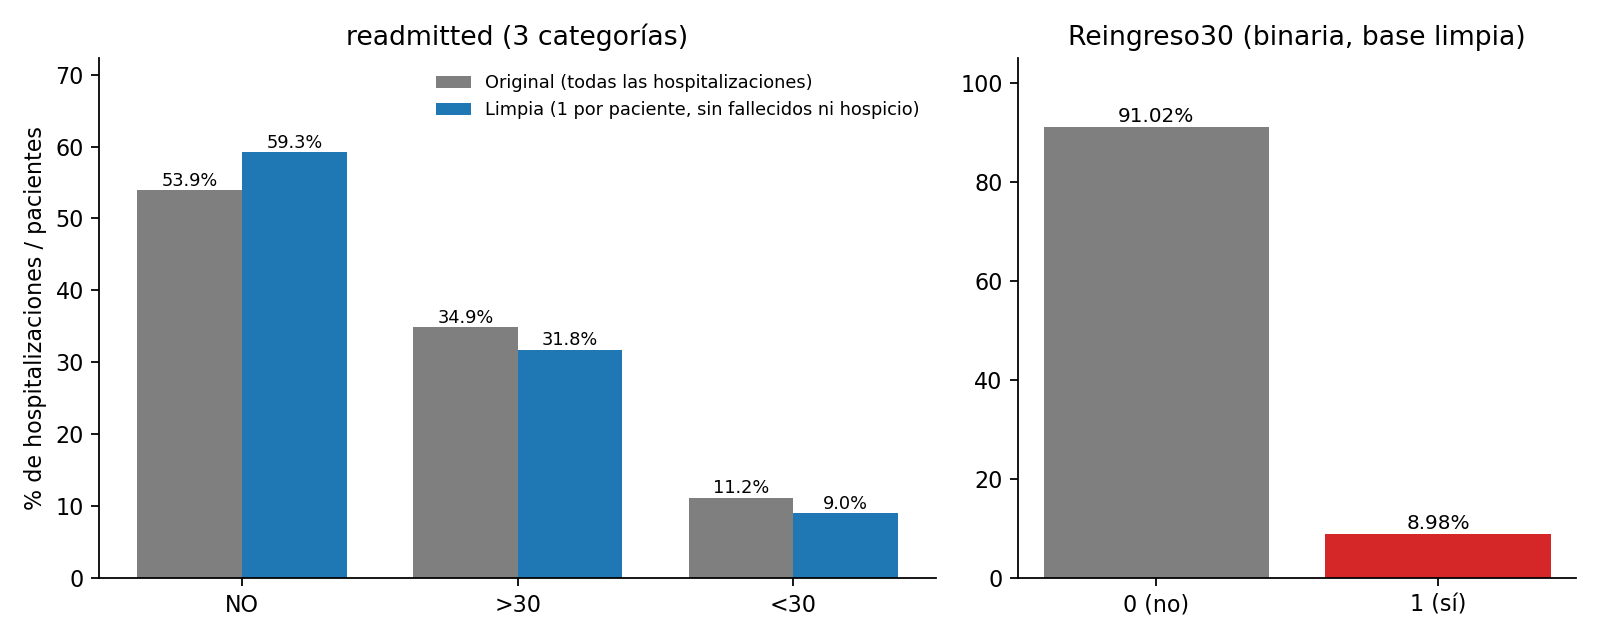
\includegraphics[width=\textwidth]{figuras/fig1_distribucion.png}
\caption{Distribución de \cod{readmitted} (original y limpia) y de \cod{Reingreso30}.}\label{fig:dist}\end{figure}
\begin{tablaentex}{Distribución de \cod{readmitted} antes de la limpieza y de \cod{readmitted} y \cod{Reingreso30} después.}{tab:dist}
\begin{tabular}{lllrr}
\toprule
base & variable & categoria & n & porcentaje \\
\midrule
original & readmitted & \textless{}30 & 11\,357 & 11.16 \\
original & readmitted & \textgreater{}30 & 35\,545 & 34.93 \\
original & readmitted & NO & 54\,864 & 53.91 \\
limpia & readmitted & \textless{}30 & 6\,285 & 8.98 \\
limpia & readmitted & \textgreater{}30 & 22\,226 & 31.76 \\
limpia & readmitted & NO & 41\,479 & 59.26 \\
limpia & Reingreso30 & 0 & 63\,705 & 91.02 \\
limpia & Reingreso30 & 1 & 6\,285 & 8.98 \\
\bottomrule
\end{tabular}
\end{tablaentex}

\paragraph{Datos faltantes.} La tabla~\ref{tab:falt} muestra las cinco columnas con más celdas vacías tras la limpieza. \cod{weight} (96.02\,\%) es inutilizable; \cod{medical\_specialty} (48.08\,\%) y \cod{payer\_code} (43.46\,\%) faltan en casi la mitad de los registros y, probablemente, no al azar (dependen de las prácticas de cada hospital), por lo que no se usan como predictores. \cod{admission\_type\_id} (11.28\,\%) y \cod{admission\_source\_id} (7.24\,\%) se tratan como una categoría adicional \cod{NA} en el Modelo B. Además, los exámenes de laboratorio casi no se realizan (tabla~\ref{tab:noexam}): 81.65\,\% sin HbA1c y 95.22\,\% sin glucosa sérica. Que el examen no se haga no es un dato faltante, pero limita lo que el resultado puede aportar: \cod{A1Cresult} entra al Modelo B con \cod{None} como categoría propia, y \cod{max\_glu\_serum} no se usa.
\begin{tablaentex}{Las cinco columnas con mayor porcentaje de celdas vacías en \cod{diab\_clean.csv}.}{tab:falt}
\begin{tabular}{lrr}
\toprule
columna & faltantes & pct\_faltante \\
\midrule
weight & 67\,202 & 96.02 \\
medical\_specialty & 33\,654 & 48.08 \\
payer\_code & 30\,416 & 43.46 \\
admission\_type\_id & 7\,893 & 11.28 \\
admission\_source\_id & 5\,069 & 7.24 \\
\bottomrule
\end{tabular}
\end{tablaentex}
\begin{tablaentex}{Exámenes no realizados (\cod{None}); no se consideran datos faltantes.}{tab:noexam}
\begin{tabular}{lrr}
\toprule
columna & filas\_con\_None & pct\_examen\_no\_realizado \\
\midrule
A1Cresult & 57\,144 & 81.65 \\
max\_glu\_serum & 66\,641 & 95.22 \\
\bottomrule
\end{tabular}
\end{tablaentex}

\paragraph{Estadísticos descriptivos.} \cod{time\_in\_hospital} y \cod{num\_medications} tienen cola derecha (media mayor que la mediana; máximos de 14 días y 81 medicamentos), mientras que \cod{num\_lab\_procedures} y \cod{number\_diagnoses} tienen medias algo menores que sus medianas. La estadía mediana es de 3.0 días (Q1--Q3: 2.0--6.0).
\begin{tablaentex}{Estadísticos descriptivos de variables numéricas seleccionadas.}{tab:desc}
\begin{tabular}{lrrrrrrrr}
\toprule
variable & n & media & desv\_est & min & Q1 & mediana & Q3 & max \\
\midrule
time\_in\_hospital & 69\,990 & 4.27 & 2.93 & 1 & 2.0 & 3.0 & 6.0 & 14 \\
num\_lab\_procedures & 69\,990 & 42.88 & 19.89 & 1 & 31.0 & 44.0 & 57.0 & 132 \\
num\_medications & 69\,990 & 15.67 & 8.29 & 1 & 10.0 & 14.0 & 20.0 & 81 \\
number\_diagnoses & 69\,990 & 7.22 & 2.00 & 1 & 6.0 & 8.0 & 9.0 & 16 \\
\bottomrule
\end{tabular}
\end{tablaentex}

\paragraph{Tasas de reingreso.} Las tablas~\ref{tab:edad}--\ref{tab:dm} y la figura~\ref{fig:tasas} muestran la tasa de reingreso a 30 días según edad, ingresos hospitalarios previos, resultado de HbA1c, cambio de medicación y uso de medicamentos para la diabetes.
\begin{figure}[H]\centering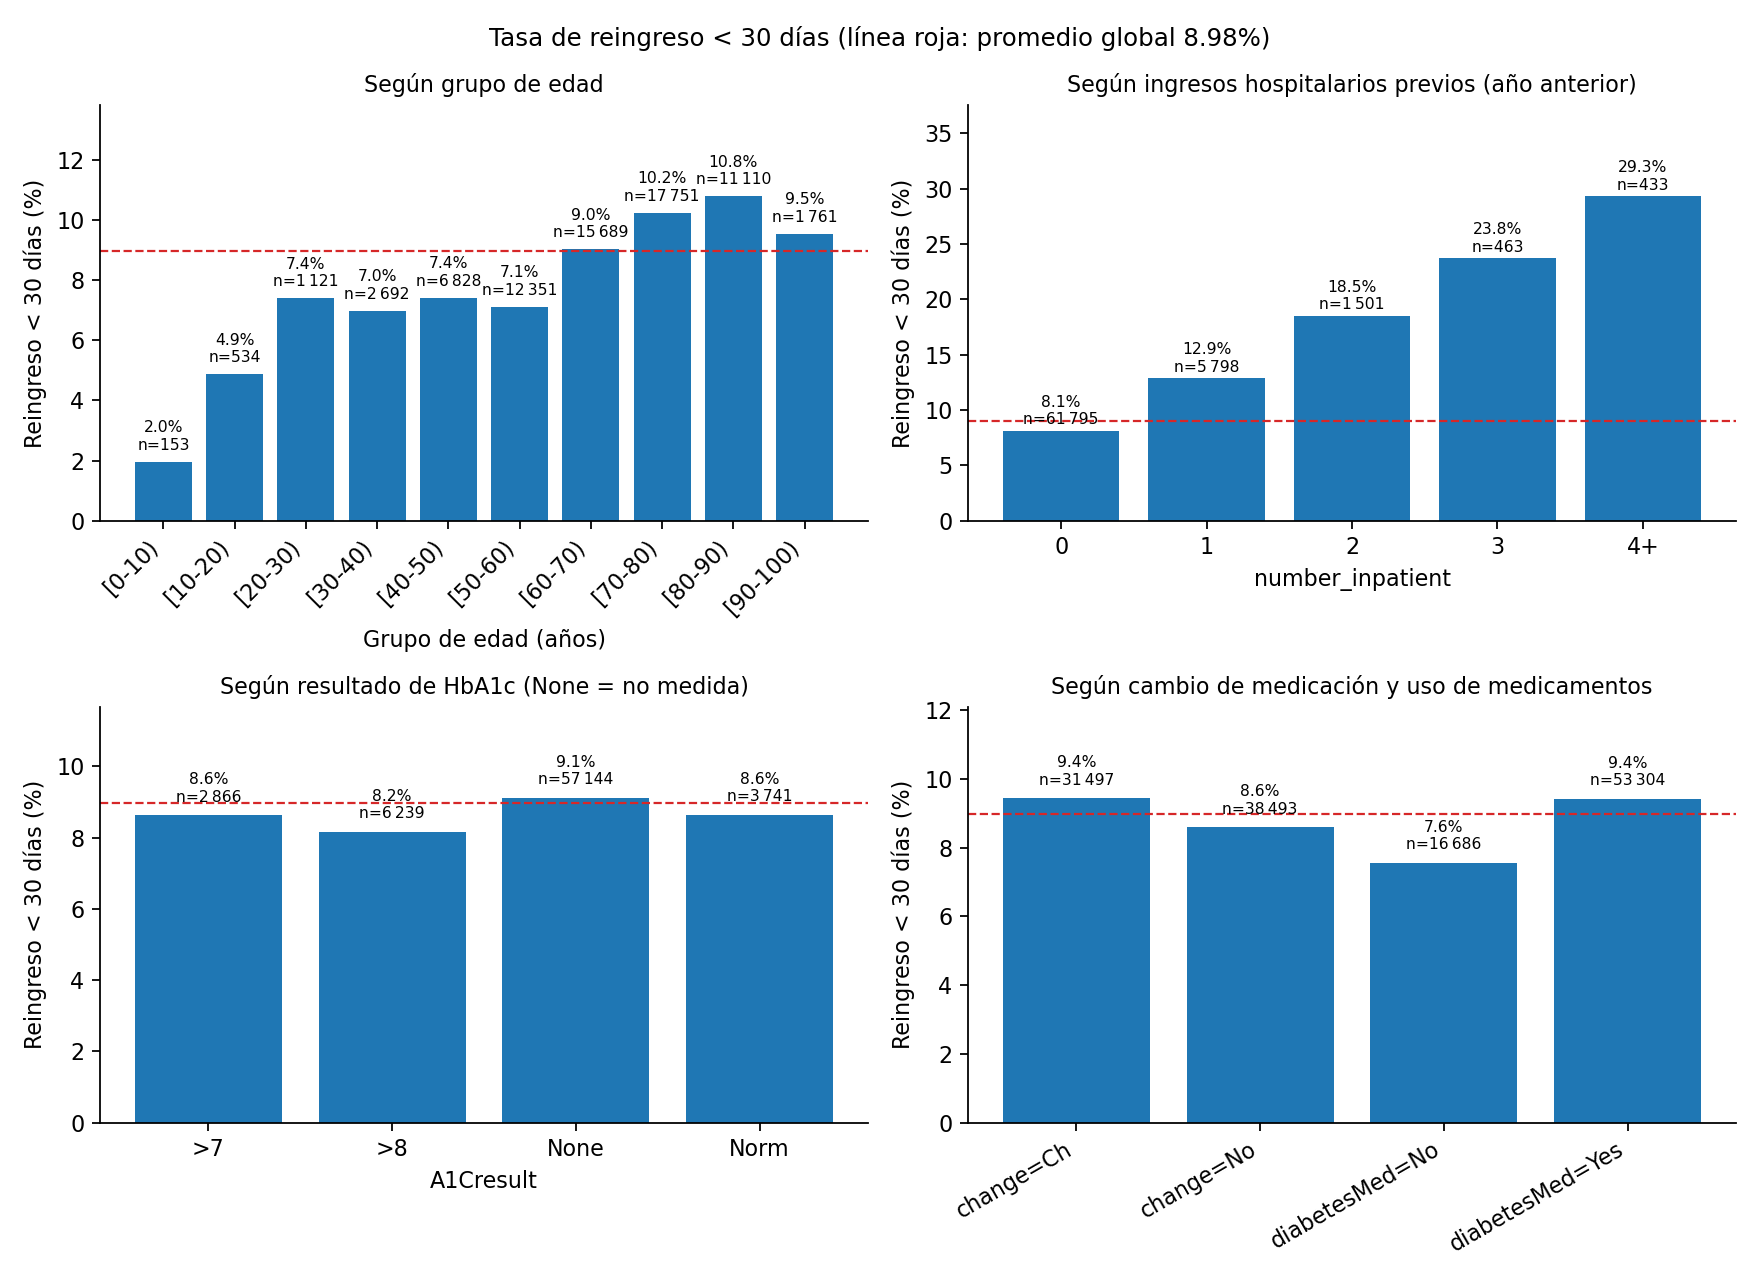
\includegraphics[width=\textwidth]{figuras/fig2_tasas.png}
\caption{Tasa de reingreso $<30$ días según variables clave (línea roja: promedio global).}\label{fig:tasas}\end{figure}
\begin{tablaentex}{Tasa de reingreso $<30$ días por grupo de edad.}{tab:edad}
\begin{tabular}{lrrr}
\toprule
grupo\_edad & n & reingresos & tasa\_pct \\
\midrule
{[}0-10) & 153 & 3 & 1.96 \\
{[}10-20) & 534 & 26 & 4.87 \\
{[}20-30) & 1\,121 & 83 & 7.40 \\
{[}30-40) & 2\,692 & 188 & 6.98 \\
{[}40-50) & 6\,828 & 506 & 7.41 \\
{[}50-60) & 12\,351 & 880 & 7.12 \\
{[}60-70) & 15\,689 & 1\,415 & 9.02 \\
{[}70-80) & 17\,751 & 1\,817 & 10.24 \\
{[}80-90) & 11\,110 & 1\,199 & 10.79 \\
{[}90-100) & 1\,761 & 168 & 9.54 \\
\bottomrule
\end{tabular}
\end{tablaentex}
\begin{tablaentex}{Tasa de reingreso $<30$ días según ingresos hospitalarios previos (\cod{number\_inpatient}).}{tab:inp}
\begin{tabular}{lrrr}
\toprule
ingresos\_previos & n & reingresos & tasa\_pct \\
\midrule
0 & 61\,795 & 5\,023 & 8.13 \\
1 & 5\,798 & 747 & 12.88 \\
2 & 1\,501 & 278 & 18.52 \\
3 & 463 & 110 & 23.76 \\
4+ & 433 & 127 & 29.33 \\
\bottomrule
\end{tabular}
\end{tablaentex}
\begin{tablaentex}{Tasa de reingreso $<30$ días según \cod{A1Cresult} (\cod{None}: no medida).}{tab:a1c}
\begin{tabular}{lrrr}
\toprule
A1Cresult & n & reingresos & tasa\_pct \\
\midrule
\textgreater{}7 & 2\,866 & 247 & 8.62 \\
\textgreater{}8 & 6\,239 & 509 & 8.16 \\
None & 57\,144 & 5\,206 & 9.11 \\
Norm & 3\,741 & 323 & 8.63 \\
\bottomrule
\end{tabular}
\end{tablaentex}
\begin{tablaentex}{Tasa de reingreso $<30$ días según cambio de medicación (\cod{change}).}{tab:ch}
\begin{tabular}{lrrr}
\toprule
change & n & reingresos & tasa\_pct \\
\midrule
Ch & 31\,497 & 2\,973 & 9.44 \\
No & 38\,493 & 3\,312 & 8.60 \\
\bottomrule
\end{tabular}
\end{tablaentex}
\begin{tablaentex}{Tasa de reingreso $<30$ días según uso de medicamentos para la diabetes (\cod{diabetesMed}).}{tab:dm}
\begin{tabular}{lrrr}
\toprule
diabetesMed & n & reingresos & tasa\_pct \\
\midrule
No & 16\,686 & 1\,262 & 7.56 \\
Yes & 53\,304 & 5\,023 & 9.42 \\
\bottomrule
\end{tabular}
\end{tablaentex}

\paragraph{Diagnósticos principales.} La tabla~\ref{tab:diag} y la figura~\ref{fig:diag} muestran los diez diagnósticos principales (\cod{diag\_1}) más frecuentes. Entre ellos, la tasa de reingreso va de 5.10\,\% (786, síntomas respiratorios y del tórax) a 16.44\,\% (434, oclusión de arterias cerebrales) y 11.47\,\% (428, insuficiencia cardiaca). La tabla usa los códigos tal como vienen, como pide el enunciado. La diabetes misma (ICD-9 250.xx) no aparece porque está repartida en 34 subcódigos. Agrupada en su categoría de tres caracteres suma 5\,748 pacientes, con una tasa de 9.12\,\%, y ocuparía el lugar 1 del ranking.
\begin{tablaentex}{Diez diagnósticos principales más frecuentes (\cod{diag\_1}, ICD-9) y su tasa de reingreso.}{tab:diag}
\begin{tabular}{rlrrr}
\toprule
diag\_1 & descripcion & n & reingresos & tasa\_pct \\
\midrule
414 & Otras formas de cardiopatía isquémica crónica & 5\,210 & 405 & 7.77 \\
428 & Insuficiencia cardiaca & 3\,879 & 445 & 11.47 \\
786 & Síntomas respiratorios y del tórax & 3\,040 & 155 & 5.10 \\
410 & Infarto agudo de miocardio & 2\,775 & 258 & 9.30 \\
486 & Neumonía (organismo no especificado) & 2\,364 & 180 & 7.61 \\
427 & Arritmias cardiacas & 2\,019 & 141 & 6.98 \\
715 & Osteoartrosis & 1\,907 & 184 & 9.65 \\
434 & Oclusión de arterias cerebrales & 1\,515 & 249 & 16.44 \\
682 & Celulitis y absceso & 1\,463 & 105 & 7.18 \\
780 & Síntomas generales & 1\,409 & 106 & 7.52 \\
\bottomrule
\end{tabular}
\end{tablaentex}
\begin{figure}[H]\centering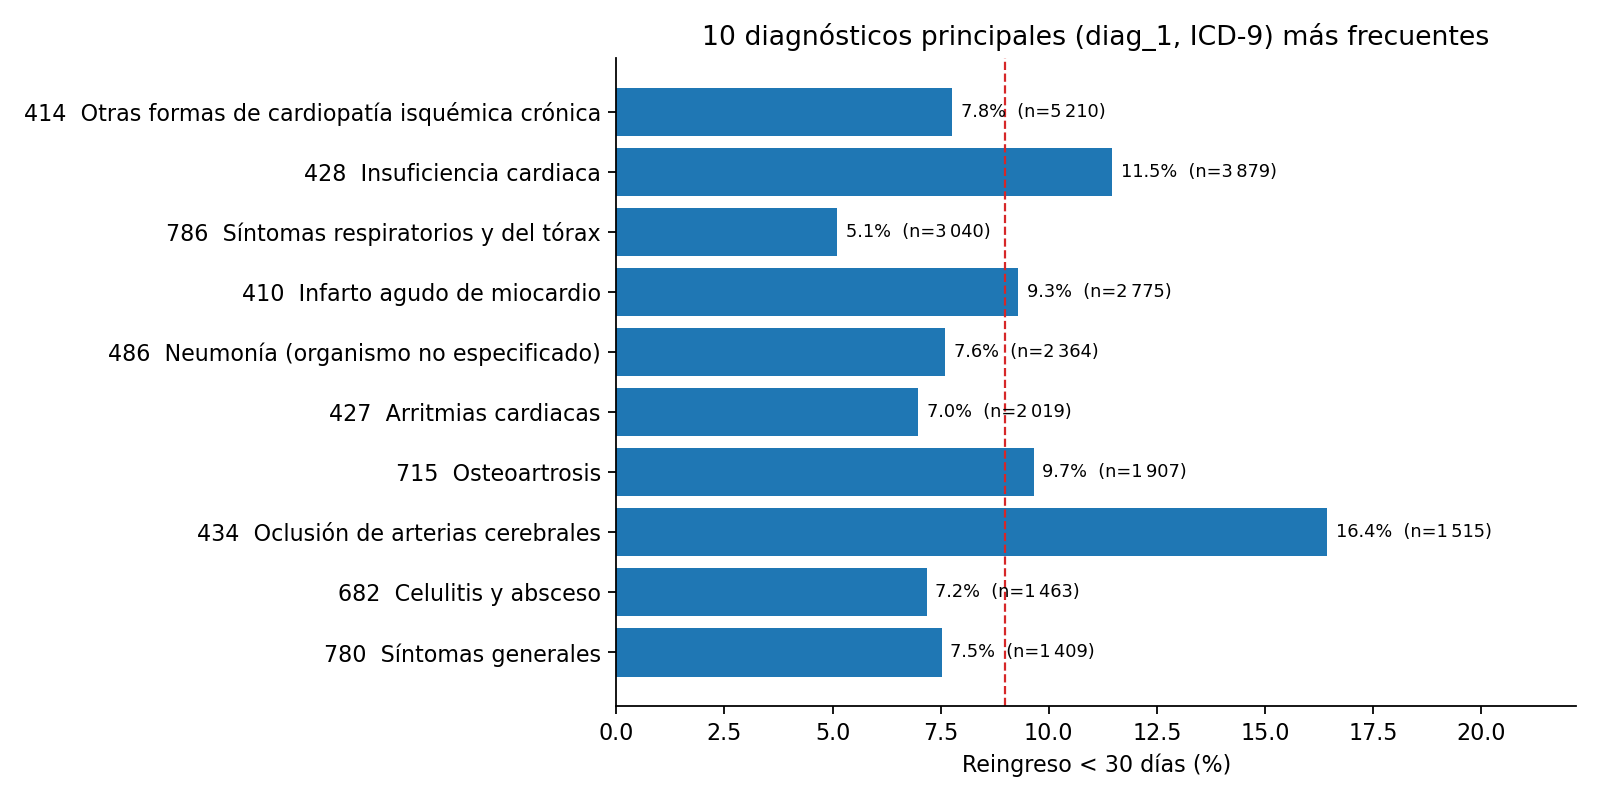
\includegraphics[width=0.95\textwidth]{figuras/fig3_diagnosticos.png}
\caption{Diagnósticos principales y tasa de reingreso $<30$ días.}\label{fig:diag}\end{figure}

\paragraph{Tres hallazgos clave.}
\begin{enumerate}
\item \textbf{Las hospitalizaciones previas son el mayor gradiente de riesgo.} La tasa sube de 8.13\,\% sin ingresos previos a 12.88\,\%, 18.52\,\%, 23.76\,\% y 29.33\,\% con 1, 2, 3 y 4 o más ($\times$3.6 entre extremos). Quienes tuvieron al menos un ingreso previo son el 11.71\,\% de los pacientes pero concentran el 20.08\,\% de los reingresos (figura~\ref{fig:tasas}, tabla~\ref{tab:inp}).
\item \textbf{El riesgo aumenta con la edad.} Entre 20 y 59 años la tasa ronda 6.98--7.41\,\%; sube a 9.02\,\% a los 60--69 y a 10.24\,\% y 10.79\,\% a los 70--79 y 80--89 años. Bajo los 20 años hay pocos casos ($n=153$ y $534$), por lo que esas tasas son inestables.
\item \textbf{El diagnóstico principal y el manejo de la diabetes separan menos que el historial.} Las variables de manejo asocian diferencias modestas (menos de 2 puntos): 9.42\,\% con medicación frente a 7.56\,\% sin ella; 9.44\,\% con cambio de medicación frente a 8.60\,\% sin cambio; y 9.11\,\% cuando la HbA1c no se midió frente a 8.16--8.63\,\% cuando sí. Son asociaciones, no efectos causales.
\end{enumerate}

\subsection{Modelación predictiva}\label{sec:resmodelos}
\paragraph{Partición.}\label{sec:resparticion}
La partición del enunciado, \cod{shuf --random-source=<(yes 42)}, \emph{no mezcla uniformemente}: el flujo \cod{42\textbackslash n42\textbackslash n\dots} es periódico y el 32.04\,\% del conjunto de prueba proviene del último decil de \cod{diab\_clean.csv} (ordenado por \cod{encounter\_id}), cuando lo esperable es 10\,\%. Como la tasa de reingreso del último decil (5.59\,\%) es menor que la del primero (9.67\,\%), la prueba queda sesgada: 9.44\,\% de reingreso en entrenamiento frente a 7.91\,\% en prueba. La partición principal (8.97\,\% frente a 9.01\,\%) usa una fuente aleatoria de calidad con la misma semilla; el entrenamiento tiene 48\,993 pacientes y la prueba 20\,997 (el 20\,\% son $K=4\,199$ pacientes). Se verificó con \cod{comm} que no hay pacientes compartidos entre ambos conjuntos.
\begin{tablaentex}{Porcentaje del conjunto de prueba proveniente de cada decil de \cod{diab\_clean.csv} con cada fuente aleatoria (esperado: 10\,\%) y tasa de reingreso del decil.}{tab:diagpart}
\begin{tabular}{rrrr}
\toprule
decil\_encounter\_id & pct\_test\_yes42 & pct\_test\_principal & tasa\_reingreso\_pct \\
\midrule
1 & 6.18 & 9.82 & 9.67 \\
2 & 5.82 & 10.03 & 10.07 \\
3 & 1.59 & 10.05 & 9.87 \\
4 & 2.77 & 10.01 & 9.62 \\
5 & 5.82 & 10.09 & 10.46 \\
6 & 6.97 & 9.81 & 9.47 \\
7 & 4.52 & 10.29 & 9.04 \\
8 & 13.55 & 10.26 & 8.13 \\
9 & 20.75 & 9.83 & 7.87 \\
10 & 32.04 & 9.82 & 5.59 \\
\bottomrule
\end{tabular}
\end{tablaentex}

\textbf{¿Por qué el final del archivo tiene menos reingresos?} No es una tendencia temporal general. Con \emph{todas} las hospitalizaciones la tasa se mantiene estable entre deciles (10.80--12.31\,\%, tabla~\ref{tab:compdec}); la caída aparece solo en la primera hospitalización de cada paciente. La explicación está en la ventana de observación. Los pacientes con más de una hospitalización registrada reingresan mucho más (20.53--30.98\,\% en todos los deciles) que los que tienen una sola (2.25--6.17\,\%). Un paciente que aparece por primera vez al final del período tiene menos tiempo para acumular hospitalizaciones dentro de los datos: en el último decil solo el 10.40\,\% tiene otra hospitalización registrada, contra 16.37--31.92\,\% en los demás. Una partición que concentra la prueba en ese decil evalúa el modelo en una población distinta de la de entrenamiento.
\begin{tablaentex}{Composición por decil de \cod{encounter\_id}: tasa de reingreso con todas las hospitalizaciones y con la primera de cada paciente, hospitalizaciones registradas por paciente, \% con otra hospitalización registrada y tasa según tengan una o varias.}{tab:compdec}
\begin{tabular}{rrrrrrr}
\toprule
decil\_encounter\_id & tasa\_todas\_hosp\_pct & tasa\_primera\_hosp\_pct & hosp\_por\_paciente & pct\_con\_otra\_hosp & tasa\_una\_hosp\_pct & tasa\_varias\_hosp\_pct \\
\midrule
1 & 11.11 & 9.67 & 1.59 & 29.72 & 5.08 & 20.53 \\
2 & 12.12 & 10.07 & 1.39 & 23.73 & 5.00 & 26.37 \\
3 & 12.03 & 9.87 & 1.22 & 16.37 & 5.74 & 30.98 \\
4 & 10.95 & 9.62 & 1.35 & 19.25 & 5.80 & 25.61 \\
5 & 12.31 & 10.46 & 1.63 & 29.80 & 6.17 & 20.57 \\
6 & 11.45 & 9.47 & 1.68 & 31.92 & 3.63 & 21.93 \\
7 & 11.02 & 9.04 & 1.48 & 25.85 & 3.22 & 25.76 \\
8 & 11.16 & 8.13 & 1.44 & 25.98 & 3.20 & 22.17 \\
9 & 10.93 & 7.87 & 1.29 & 20.46 & 2.25 & 29.75 \\
10 & 10.80 & 5.59 & 1.13 & 10.40 & 2.74 & 30.08 \\
\bottomrule
\end{tabular}
\end{tablaentex}

\paragraph{Desempeño en el 20\,\% de mayor riesgo.}
\begin{tablaentex}{Resultados en el conjunto de prueba (partición principal). Sensibilidad, precisión y exactitud en \%.}{tab:res}
\begin{tabular}{lrrrrrrr}
\toprule
modelo & capturados\_top20 & reingresos\_test & sensibilidad\_pct & precision\_pct & lift & auc & exactitud\_pct \\
\midrule
Selección aleatoria (esperado) & 378.4 & 1\,892 & 20.00 & 9.01 & 1.00 & 0.500 & - \\
Modelo A & 552 & 1\,892 & 29.18 & 13.15 & 1.46 & 0.593 & 90.98 \\
Modelo B & 702 & 1\,892 & 37.10 & 16.72 & 1.86 & 0.648 & 90.97 \\
Siempre no reingreso & 0 & 1\,892 & 0.00 & - & - & - & 90.99 \\
\bottomrule
\end{tabular}
\end{tablaentex}
El \textbf{Modelo B} captura 702 de los 1\,892 reingresos de la prueba contactando al 20\,\% (37.10\,\%), con precisión 16.72\,\% y \emph{lift} 1.86; el Modelo A captura 29.18\,\% (\emph{lift} 1.46). La selección aleatoria captura 20\,\%: en 1000 simulaciones de selección aleatoria del 20\,\% la sensibilidad media fue 19.97\,\% (desviación estándar 0.86; rango 16.86--22.89\,\%). La exactitud de predecir siempre «no reingreso» es 90.99\,\%, prácticamente igual a la de los modelos con umbral 0.5 (90.98\,\% y 90.97\,\%).
\begin{figure}[H]\centering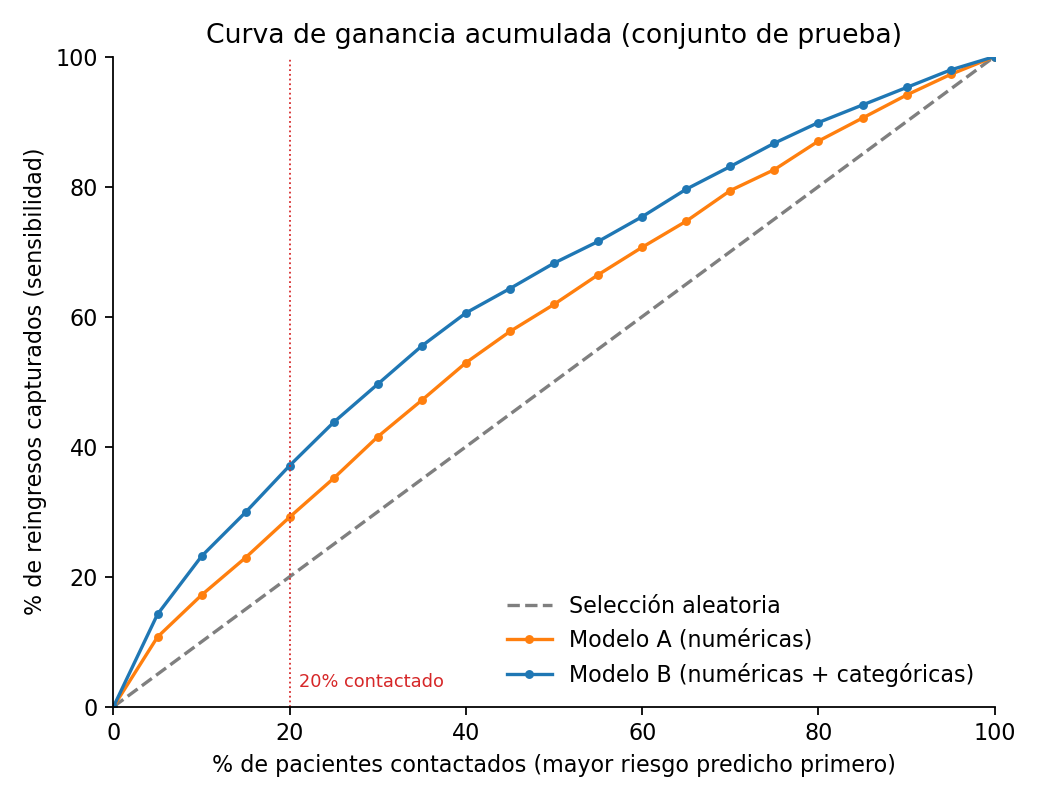
\includegraphics[width=0.62\textwidth]{figuras/fig4_ganancia.png}
\caption{Curva de ganancia acumulada en el conjunto de prueba.}\label{fig:gan}\end{figure}
\begin{tablaentex}{Intervalos de confianza del 95\,\% (\emph{bootstrap}) para sensibilidad (\%) y \emph{lift} en el 20\,\% superior, y diferencias B menos A.}{tab:bs}
\begin{tabular}{lrrr}
\toprule
metrica & ic95\_inf & mediana & ic95\_sup \\
\midrule
sensibilidad\_A & 27.17 & 29.19 & 31.10 \\
sensibilidad\_B & 34.94 & 37.13 & 39.33 \\
lift\_A & 1.36 & 1.46 & 1.55 \\
lift\_B & 1.76 & 1.86 & 1.96 \\
dif\_sensibilidad\_B\_menos\_A & 5.79 & 7.95 & 10.11 \\
dif\_lift\_B\_menos\_A & 0.30 & 0.40 & 0.50 \\
\bottomrule
\end{tabular}
\end{tablaentex}
Estos intervalos reflejan solo la variabilidad del conjunto de prueba, con los modelos ya entrenados. No incluyen la variabilidad del entrenamiento (otra partición daría otros pesos), por lo que subestiman la incertidumbre total. La comparación con la partición del enunciado (tabla~\ref{tab:comp}) da una idea de esa otra fuente de variación.
\begin{tablaentex}{Sensibilidad de los resultados a la partición: principal frente a la del enunciado (\cod{yes 42}).}{tab:comp}
\begin{tabular}{lrrrrrr}
\toprule
particion & tasa\_train\_pct & tasa\_test\_pct & sens\_A\_pct & lift\_A & sens\_B\_pct & lift\_B \\
\midrule
principal & 8.97 & 9.01 & 29.18 & 1.46 & 37.10 & 1.86 \\
enunciado & 9.44 & 7.91 & 27.59 & 1.38 & 34.46 & 1.72 \\
\bottomrule
\end{tabular}
\end{tablaentex}
Las conclusiones son cualitativamente iguales con ambas particiones (B supera a A y ambos superan al azar), pero la partición del enunciado entrega un conjunto de prueba con una tasa de reingreso distinta de la de entrenamiento, por lo que sus cifras no son directamente comparables.

\paragraph{Pesos del modelo.}
Las tablas~\ref{tab:wnum} y~\ref{tab:wtop} y la figura~\ref{fig:pesos} muestran los pesos del Modelo B: las numéricas están estandarizadas (peso por una desviación estándar) y los pesos de las variables categóricas se expresan como contraste con su categoría de referencia (la más frecuente); la interpretación se discute en la sección~\ref{sec:disc}.
\begin{tablaentex}{Modelo B: pesos de las variables numéricas (por una desviación estándar).}{tab:wnum}
\begin{tabular}{lr}
\toprule
variable & peso\_por\_DE \\
\midrule
time\_in\_hospital & 0.053 \\
num\_lab\_procedures & 0.047 \\
num\_procedures & $-$0.007 \\
num\_medications & 0.000 \\
number\_outpatient & $-$0.002 \\
number\_emergency & 0.025 \\
number\_inpatient & 0.194 \\
number\_diagnoses & 0.073 \\
\bottomrule
\end{tabular}
\end{tablaentex}
\begin{tablaentex}{Modelo B: 15 mayores efectos entre variables numéricas y categorías con $n\geq300$ en el entrenamiento (categóricas relativas a la categoría de referencia, la más frecuente).}{tab:wtop}
\begin{tabular}{llllrrl}
\toprule
variable & nivel & descripcion & referencia & n\_train & peso & tipo \\
\midrule
discharge\_disposition\_id & 22 & Discharged/transferred to another rehab fac... & 1 & 971 & 1.399 & categórica vs referencia \\
discharge\_disposition\_id & 5 & Discharged/transferred to another type of i... & 1 & 645 & 1.114 & categórica vs referencia \\
discharge\_disposition\_id & 2 & Discharged/transferred to another short ter... & 1 & 1\,081 & 0.698 & categórica vs referencia \\
discharge\_disposition\_id & 3 & Discharged/transferred to SNF & 1 & 6\,172 & 0.495 & categórica vs referencia \\
age & {[}10-20) &  & {[}70-80) & 369 & $-$0.381 & categórica vs referencia \\
discharge\_disposition\_id & 4 & Discharged/transferred to ICF & 1 & 376 & 0.348 & categórica vs referencia \\
discharge\_disposition\_id & NA &  & 1 & 2\,288 & 0.340 & categórica vs referencia \\
admission\_source\_id & 5 & Transfer from a Skilled Nursing Facility (SNF) & 7 & 358 & $-$0.274 & categórica vs referencia \\
age & {[}50-60) &  & {[}70-80) & 8\,658 & $-$0.266 & categórica vs referencia \\
diabetesMed & No &  & Yes & 11\,776 & $-$0.263 & categórica vs referencia \\
age & {[}90-100) &  & {[}70-80) & 1\,235 & $-$0.203 & categórica vs referencia \\
age & {[}30-40) &  & {[}70-80) & 1\,856 & $-$0.201 & categórica vs referencia \\
number\_inpatient &  &  &  &  & 0.194 & numérica (por 1 DE) \\
insulin & Down &  & No & 5\,035 & 0.185 & categórica vs referencia \\
discharge\_disposition\_id & 6 & Discharged/transferred to home with home he... & 1 & 5\,802 & 0.178 & categórica vs referencia \\
\bottomrule
\end{tabular}
\end{tablaentex}
\begin{figure}[H]\centering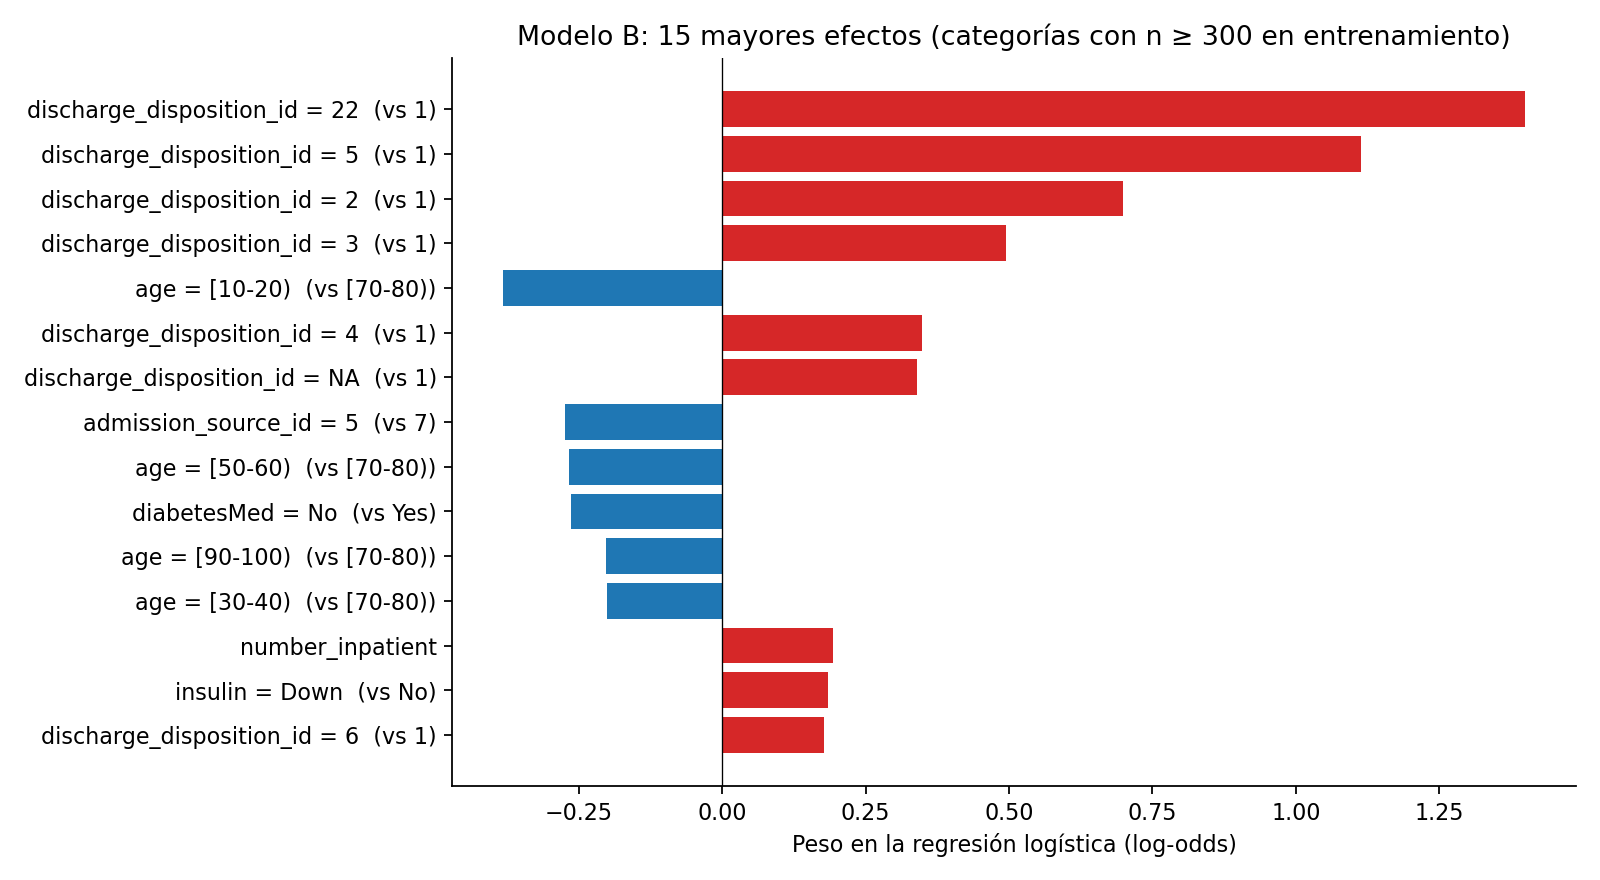
\includegraphics[width=0.95\textwidth]{figuras/fig5_pesos.png}
\caption{Modelo B: mayores pesos (log-odds).}\label{fig:pesos}\end{figure}

\subsection{Desempeño por grupo racial}\label{sec:equidad}
La raza no es predictor de ningún modelo, pero se auditó el desempeño del Modelo B por grupo (tabla~\ref{tab:eq}, figura~\ref{fig:eq}). Con tasas de reingreso observadas de 9.20\,\% en caucásicos y 8.36\,\% en afroamericanos, el modelo incluye en el 20\,\% de mayor riesgo al 21.33\,\% de los caucásicos (IC 95\,\%: 20.7-22.0) y al 15.45\,\% de los afroamericanos (IC 95\,\%: 14.3-16.6), una brecha estadísticamente clara, con intervalos disjuntos; captura 37.88\,\% (IC 95\,\%: 35.4-40.4) de los reingresos de los primeros frente a 31.55\,\% (26.4-36.7) de los segundos, una brecha no concluyente, con intervalos que se solapan. Es un chequeo exploratorio: los intervalos son de Wald y varios grupos son pequeños.
\begin{tablaentex}{Modelo B por raza en el 20\,\% de mayor riesgo (\emph{NA}: raza no informada). Intervalos de Wald al 95\,\%.}{tab:eq}
\begin{tabular}{lrrrrlrlr}
\toprule
raza & n & pct\_muestra & tasa\_reingreso\_pct & pct\_seleccionado & ic95\_seleccionado & sensibilidad\_pct & ic95\_sensibilidad & precision\_pct \\
\midrule
Caucasian & 15\,701 & 74.78 & 9.20 & 21.33 & 20.7-22.0 & 37.88 & 35.4-40.4 & 16.33 \\
AfricanAmerican & 3\,794 & 18.07 & 8.36 & 15.45 & 14.3-16.6 & 31.55 & 26.4-36.7 & 17.06 \\
NA & 572 & 2.72 & 8.22 & 16.43 & 13.4-19.5 & 38.30 & 24.4-52.2 & 19.15 \\
Hispanic & 478 & 2.28 & 9.83 & 17.15 & 13.8-20.5 & 42.55 & 28.4-56.7 & 24.39 \\
Other & 335 & 1.60 & 8.66 & 17.91 & 13.8-22.0 & 41.38 & 23.5-59.3 & 20.00 \\
Asian & 117 & 0.56 & 6.84 & 23.93 & 16.2-31.7 & 62.50 & 29.0-96.0 & 17.86 \\
\bottomrule
\end{tabular}
\end{tablaentex}
\begin{figure}[H]\centering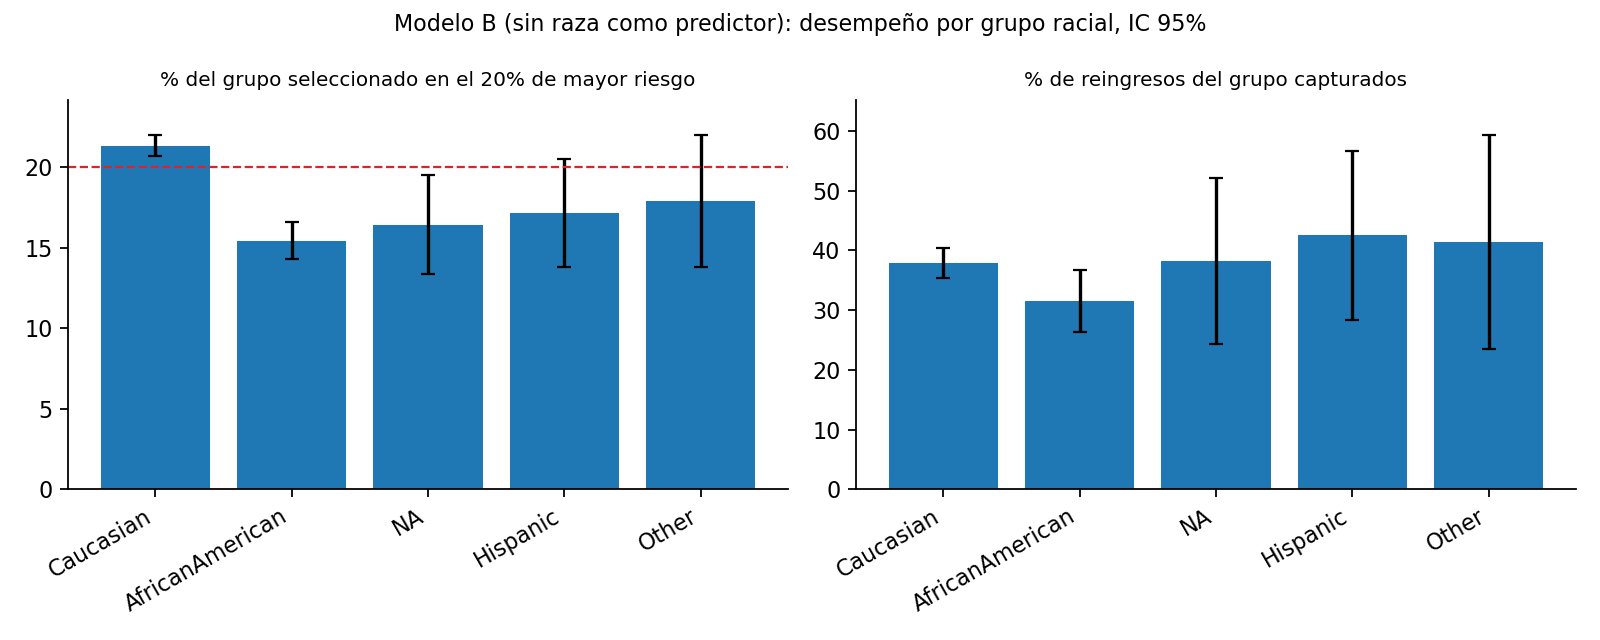
\includegraphics[width=\textwidth]{figuras/fig6_equidad.png}
\caption{Proporción seleccionada y sensibilidad por raza (grupos con $n\geq300$), IC 95\,\%.}\label{fig:eq}\end{figure}

\textbf{¿De dónde viene la brecha de selección?} La tabla~\ref{tab:eqcomp} compara la composición de cada grupo en las variables de mayor peso del Modelo B. El 29.26\,\% de los pacientes afroamericanos tiene 70 años o más, contra 47.92\,\% de los caucásicos. Tienen algún ingreso previo el 9.52\,\% contra el 12.15\,\%, y son dados de alta a otra institución (códigos 2, 3, 4, 5 y 22) el 14.55\,\% contra el 20.11\,\%. Entre los seleccionados, la precisión es similar: 17.06\,\% (IC 95\,\%: 14.0-20.1) contra 16.33\,\% (15.1-17.6), una diferencia no concluyente, con intervalos que se solapan.
\begin{tablaentex}{Composición de los pacientes de prueba por raza y precisión del Modelo B entre los seleccionados (IC 95\,\% de Wald).}{tab:eqcomp}
\begin{tabular}{lrrrrrrrl}
\toprule
raza & n & edad\_70\_o\_mas\_pct & ingreso\_previo\_pct & alta\_a\_institucion\_pct & tasa\_reingreso\_pct & pct\_seleccionado & precision\_pct & ic95\_precision \\
\midrule
Caucasian & 15\,701 & 47.92 & 12.15 & 20.11 & 9.20 & 21.33 & 16.33 & 15.1-17.6 \\
AfricanAmerican & 3\,794 & 29.26 & 9.52 & 14.55 & 8.36 & 15.45 & 17.06 & 14.0-20.1 \\
NA & 572 & 40.91 & 8.04 & 18.71 & 8.22 & 16.43 & 19.15 & 11.2-27.1 \\
Hispanic & 478 & 26.15 & 13.81 & 12.97 & 9.83 & 17.15 & 24.39 & 15.1-33.7 \\
Other & 335 & 31.64 & 10.45 & 14.63 & 8.66 & 17.91 & 20.00 & 9.9-30.1 \\
Asian & 117 & 54.70 & 10.26 & 21.37 & 6.84 & 23.93 & 17.86 & 3.7-32.0 \\
\bottomrule
\end{tabular}
\end{tablaentex}

% ------------------------------------------------------------------ 5
\section{Discusión}\label{sec:disc}
\paragraph{(i) ¿Qué modelo prioriza mejor y cuánto mejora respecto de la selección aleatoria?}
El Modelo B. Contactando al 20\,\% de mayor riesgo captura 37.10\,\% de los reingresos frente a 20\,\% del azar, es decir, 1.86 veces lo que capturaría una selección aleatoria (IC 95\,\% del \emph{lift}: 1.76--1.96); el Modelo A llega a 29.18\,\% (\emph{lift} 1.46). La ventaja de B sobre A es de 7.95 puntos de sensibilidad (IC 95\,\%: 5.79 a 10.11), con el intervalo completo sobre cero. El AUC es 0.648 (B) y 0.593 (A): hay señal útil para priorizar, pero el poder discriminativo es modesto.

\paragraph{(ii) ¿Por qué la exactitud es una métrica engañosa en este problema?}
Porque solo alrededor del 8.98\,\% de los pacientes reingresa: un «modelo» que siempre predice «no reingreso» logra 90.99\,\% de exactitud sin identificar a ningún paciente de riesgo (sensibilidad 0\,\%). Los modelos A y B, con umbral 0.5, tienen 90.98\,\% y 90.97\,\%, prácticamente lo mismo, porque casi ninguna probabilidad supera 0.5 (solo 13 y 17 de 20\,997 pacientes en A y B), aunque B ordena claramente mejor. La exactitud ignora el orden y el desbalance; aquí importa la capacidad de \emph{ranking} (sensibilidad, precisión y \emph{lift} en el 20\,\% superior).

\paragraph{(iii) ¿Qué variables ponderan más y son clínicamente razonables?}
Entre las numéricas (por desviación estándar), pesa más \cod{number\_inpatient} (0.194), seguida de \cod{number\_diagnoses} (0.073) y \cod{time\_in\_hospital} (\mbox{0.053}): más hospitalizaciones previas, estadías largas y más diagnósticos (mayor complejidad clínica) aumentan el riesgo. Entre las categóricas, relativas al alta a domicilio, destacan el alta a \textbf{rehabilitación} (1.399), a otro tipo de \textbf{institución de cuidado} (1.114), a \textbf{otro hospital} (0.698) y a un \textbf{centro de enfermería especializada} (0.495), que son pacientes más frágiles; los pacientes de 10 a 19 años tienen menor riesgo (\cod{age=[10-20)}: \mbox{$-$0.381} frente a 70--79 años), igual que quienes no usan medicación para la diabetes (\mbox{$-$0.263}); la insulina con dosis reducida (\cod{Down}) se asocia a mayor riesgo (\mbox{0.185}). Los pesos de las numéricas (por desviación estándar) y los de las categorías (contraste con la categoría de referencia) no son directamente comparables entre sí. La mayoría de los efectos es clínicamente razonable, con dos matices. Primero, el peso de \cod{time\_in\_hospital} baja de \mbox{0.119} en el Modelo A a \mbox{0.053} en el B: parte de su efecto lo recoge el destino al alta, porque las estadías largas terminan más a menudo en traslado a otra institución (estadía media de 5.56 días con alta a otra institución, contra 3.61 con alta a domicilio). El peso de una variable depende de qué otras incluye el modelo. Segundo, el ingreso desde un centro de enfermería especializada (\cod{admission\_source\_id=5}) tiene peso negativo (\mbox{$-$0.274}), sin una explicación clínica evidente; puede reflejar cómo se registra ese origen, y no conviene interpretarlo. En todo caso son \emph{asociaciones predictivas, no causales}, y las categorías raras ($<300$ pacientes) no deben interpretarse.

\paragraph{(iv) Efecto de usar varias hospitalizaciones de un mismo paciente y cómo verificarlo.}
Se esperan resultados \textbf{optimistas}. Las hospitalizaciones de un paciente están correlacionadas (misma edad, comorbilidades e historial de ingresos), por lo que con una partición al azar por fila el mismo paciente quedaría en entrenamiento y en prueba y el modelo lo «reconocería» (fuga de información), inflando AUC, sensibilidad y \emph{lift}; además se subestimaría la incertidumbre al tratar como independientes datos que no lo son, y los pacientes con muchas hospitalizaciones quedarían sobrerrepresentados. \emph{Verificación.} Además de comprobar con \cod{comm -12} que el análisis principal no comparte pacientes entre entrenamiento y prueba (0 compartidos), se hizo el experimento directo. Con todas las hospitalizaciones tras la exclusión (99\,343, sin deduplicar) se entrenó el mismo Modelo B con dos particiones 70/30 que solo difieren en cómo se reparte: \emph{por fila} (cada hospitalización al azar) y \emph{por paciente} (se sortean pacientes y todas sus hospitalizaciones van al mismo lado). Los resultados están en la tabla~\ref{tab:fuga}.
\begin{tablaentex}{Modelo B con todas las hospitalizaciones: partición por fila frente a partición por paciente, y el análisis principal como referencia.}{tab:fuga}
\begin{tabular}{lrrrrrrrr}
\toprule
escenario & n\_train & n\_test & pct\_test\_paciente\_en\_train & tasa\_test\_pct & sensibilidad\_B\_pct & precision\_B\_pct & lift\_B & auc\_B \\
\midrule
Una hospitalización por paciente (principal) & 48\,993 & 20\,997 & 0.00 & 9.01 & 37.10 & 16.72 & 1.86 & 0.648 \\
Todas las hospitalizaciones; partición por fila & 69\,540 & 29\,803 & 39.00 & 11.29 & 37.49 & 21.16 & 1.87 & 0.663 \\
Todas las hospitalizaciones; partición por paciente & 69\,483 & 29\,860 & 0.00 & 11.64 & 36.93 & 21.50 & 1.85 & 0.657 \\
\bottomrule
\end{tabular}
\end{tablaentex}
\emph{Resultado.} La fuga es real: con la partición por fila, el 39.00\,\% de las hospitalizaciones de prueba pertenece a pacientes que también están en entrenamiento. Pero su efecto en este modelo es pequeño: AUC 0.663 contra 0.657 (diferencia 0.006) y sensibilidad 37.49\,\% contra 36.93\,\% (diferencia 0.56 puntos), dentro de la variación esperable de una sola partición. Una regresión logística con 17 variables generales no puede memorizar pacientes; la fuga sería mucho mayor con modelos flexibles o con variables que identifiquen al paciente. El efecto más importante es otro: \textbf{cambia la población evaluada}. La tasa de reingreso de la prueba pasa de 9.01\,\% (por paciente) a 11.64\,\% (por hospitalización), y la precisión del 20\,\% superior de 16.72\,\% a 21.50\,\%, porque los pacientes recurrentes aportan muchas filas. Esas cifras miden «hospitalizaciones contactadas» y no «pacientes contactados», y sobreestimarían lo que el programa logra por cada paciente al que llama. Por eso el análisis principal usa un registro por paciente.

\paragraph{(v) ¿Es apropiado usar la raza como predictor en un programa de seguimiento?}
No. (a) La raza es un atributo protegido: usarla para decidir a quién se contacta puede producir trato desigual y riesgo legal y ético, y su asociación con el reingreso refleja determinantes sociales (acceso, seguro, vecindario) más que biología. (b) En los datos falta en 2.23\,\% de las hospitalizaciones y varios grupos son pequeños. (c) Aun sin raza el modelo no es neutral: como se vio en la sección~\ref{sec:equidad}, la proporción de pacientes seleccionados es menor en pacientes afroamericanos (brecha estadísticamente clara, con intervalos disjuntos) y también lo es la sensibilidad (brecha no concluyente, con intervalos que se solapan); la brecha de selección coincide con diferencias de composición en las variables que más pesan (edad, ingresos previos, alta a otra institución), mientras que la precisión entre los seleccionados es similar (tabla~\ref{tab:eqcomp}). (d) Esas mismas variables pueden recoger diferencias de acceso a la atención: un menor registro de ingresos previos puede reflejar menos acceso y no menos riesgo, algo que estos datos no permiten distinguir.

\textbf{Recomendación.} No usar la raza como predictor y usarla \emph{solo para auditar}: medir periódicamente, por grupo, la proporción seleccionada, la sensibilidad y la precisión. Igualar la sensibilidad entre grupos exigiría fijar cuotas o umbrales por raza, lo que en sí mismo es usar la raza para decidir a quién se llama. Es una decisión de política, con implicancias legales y éticas, que corresponde al comité y no al modelo.

% ------------------------------------------------------------------ 6
\section{Conclusiones y recomendación al comité}
\begin{itemize}
\item \textbf{Recomendación.} Usar el \textbf{Modelo B} para priorizar el seguimiento telefónico: contactar al 20\,\% de los pacientes con mayor riesgo captura \textbf{37.10\,\%} de los reingresos a 30 días, \textbf{1.86 veces} lo que se lograría al azar.
\item \textbf{Alcance.} El AUC de 0.648 indica un ordenamiento solo moderado: el 62.90\,\% de los reingresos queda fuera del 20\,\% contactado. Conviene complementar el modelo con reglas simples y trazables (ingresos previos y alta a una institución de cuidado) y evaluarlo en datos más recientes.
\item \textbf{Hallazgos descriptivos.} El historial de ingresos previos y la edad avanzada son los factores más asociados al reingreso temprano; el manejo de la diabetes y los exámenes aportan asociaciones modestas, y los exámenes casi no se realizan.
\item \textbf{Equidad y privacidad.} No usar la raza como predictor, sino solo para auditar. Monitorear por grupo la proporción seleccionada, la sensibilidad y la precisión: hoy se selecciona a una menor proporción de pacientes afroamericanos, con una precisión similar. Cualquier ajuste por grupo debe decidirlo el comité de forma explícita. No distribuir los datos fuera del entorno autorizado.
\end{itemize}

\subsection*{Limitaciones}
Un solo conjunto de prueba (sin validación cruzada ni validación temporal); intervalos \emph{bootstrap} que solo recogen la variabilidad de la prueba; ventana de observación más corta para los pacientes vistos por primera vez al final del período; modelo lineal sin interacciones y sin ajuste fino de hiperparámetros; datos de 1999--2008, de un grupo de hospitales y solo con los reingresos observados en ellos; análisis restringido a la primera hospitalización de cada paciente; \cod{encounter\_id} se usa solo como proxy del orden temporal; y las diferencias por grupo racial provienen de un único conjunto de prueba con grupos pequeños.

% ------------------------------------------------------------------ 7
\section{Reproducibilidad}
Para reproducir exactamente las salidas basta ejecutar, desde la raíz del repositorio y dentro del contenedor \cod{datasciencetoolbox/dsatcl2e} (o una terminal Linux con las herramientas indicadas):
\begin{lstlisting}
git clone https://github.com/trini-tini/evaluacion1-diabetes && cd evaluacion1-diabetes
bash scripts/pipeline.sh
\end{lstlisting}
El \emph{pipeline} descarga los datos, ejecuta la limpieza, el análisis exploratorio y la modelación, genera \cod{data/diab\_clean.csv}, las tablas intermedias (\cod{data/tablas}), las figuras (\cod{report/figuras}), la ficha (\cod{report/ficha.txt}), \cod{report/reporte.md} y este informe. La estructura del repositorio es:
\begin{lstlisting}[columns=fixed]
scripts/pipeline.sh     pipeline completo, comentado y en orden logico
scripts/graficos.py     figuras (matplotlib)
scripts/csv2tex.py      tablas CSV -> LaTeX
report/reporte.md.tpl   plantilla con marcadores de doble llave -> report/reporte.md
report/informe.tex.tpl  plantilla del informe -> report/informe.tex -> informe.pdf
report/figuras          figuras generadas
data/                   datos, particiones y tablas intermedias (no se versionan)
\end{lstlisting}

\clearpage
\appendix
\section{Ficha de seguimiento post-alta}
La ficha se genera con comandos a partir de \cod{data/diab\_clean.csv} y de \cod{data/test\_pred.csv} (Modelo B, partición principal), sin escribir los valores a mano:
\begin{lstlisting}
Comite de Calidad - Ficha de Seguimiento Post-Alta
Analista: piasa
Pacientes analizados: 69990
Reingreso en <30 dias: 8.98%
Reingresos capturados contactando al 20%: 37.10%
Lift del modelo: 1.86
\end{lstlisting}

\section{Entorno de ejecución}\label{app:entorno}
\begin{lstlisting}
fecha: 2026-10-22 18:50
sistema: Linux 6.18.33.1-microsoft-standard-WSL2
bash: 5.2.21(1)-release
awk: GNU Awk 5.2.1, API 3.2, PMA Avon 8-g1, (GNU MPFR 4.2.1, GNU MP 6.3.0)
shuf: shuf (GNU coreutils) 9.4
vw: 8.6.1
csvkit: csvstat 1.4.0
python3: Python 3.12.3 / matplotlib 3.6.3
\end{lstlisting}

\end{document}
